\documentclass{softwaremanual}

\usepackage{titling}
\usepackage{ragged2e}
\usepackage{booktabs,xcolor,siunitx}
\definecolor{lightgray}{gray}{0.95}
% Figures and controlling packages
\usepackage{float}
\usepackage{wrapfig}

% logo for the title page
%\newcommand{\swlogo}{{\includegraphics[width=0.25\textwidth]{images/shallowWater.png}}
%}


\author{Joseph Schoonover, Jiaxu Zhang, Wilbert Weijer}
\date{}

\begin{document}
\frontmatter
% Doing a custom title-page
\begin{titlingpage}
    
        \vspace*{2cm}

   % Setup up the main and sub-titles with the logo

   {\fontfamily{cmss}\selectfont
   \begin{center}
     \Large{\textbf{ Fast Equilibration of Oceanic Tracers Software  }}\\
   \end{center}
    } 
\hspace{3.2385cm} \includegraphics[width=0.7\linewidth,natwidth=9500,natheight=3300]{Logo/FEOTS_Logo.png}

     %\Large{\textbf{\textcolor{blue}{(FEOTS)}}}
      
 
        
        \vspace{2cm}
        
     \begin{center}
     
        %Do a subtitle here if you like
        { \fontfamily{cmss}\selectfont
          \large{ User's Guide and Technical Documentation }\\
          \vspace{1.5cm}
           % Enter the author's name
          \textbf{\large{\theauthor}}
          
        }
        
        \vspace{8cm}
        
        \copyright 2017 Joseph Schoonover, Los Alamos National Laboratory
     \end{center}
        
    
\end{titlingpage}

The Fast Equilibration of Ocean Tracers Software (FEOTS) is a set of Fortran modules and programs for post-processing output from LANL's Parallel Ocean Program (POP). However, it is written so that it can be extended for use with other General Circulation Models. Tools are provided for aiding in the diagnosis of sparse matrices that capture advection and diffusion operators that are consistent with GCM discretizations. FEOTS additionally offers tools to make use of the diagnosed operators to run offline tracer models in forward or equilibration modes.


 Many thanks to Wilbert Weijer and Matthew Hecht for their support on developing this software.
  
 \begin{flushright}
 - Joseph Schoonover
 \end{flushright}

\pagebreak

{\fontfamily{cmss}\selectfont
\tableofcontents*
}
\mainmatter

% Special Style
\pagestyle{myheadings}
\part{Users Guide}
\chapter{Getting Started}
\section{Overview}
 The Fast Equilibration of Ocean Tracers Software (FEOTS) is a General Circulation Model (GCM) post-processing tool for running offline passive tracer simulations. Offline passive tracer simulations are particularly attractive because they can be run on fewer computational resources than a full-fledged GCM. FEOTS operates in either forward mode or equilibration mode for performing transient simulations or for obtaining equilibrium solutions.  For large biogeochemical tracer systems, FEOTS offers a hybrid MPI-OpenMP parallelization strategy for maintaining reasonable throughput. There are also packages for tagging water masses based on ocean state variables (e.g. potential temperature, salinity, etc.) and location, for studying ocean mixing and water mass pathways.
 
% By providing interfaces for working with common GCM's (POP,MITgcm) our aim is provide a common framework for running offline tracer simulations quickly and accurately. Our future vision of the FEOTS code is to provide an online repository of transport operators diagnosed from state-of-the-art GCM's for researchers to access. For many researchers, having access to transport operators from already validated GCM simulatons reduces the startup cost for running their own tracer simulations and may also provide another level of validation..
 
\section{System Requirements and Software Dependencies}
At a minimum, you will need 750 KB of space for the FEOTS source code and a Fortran compiler. At present, FEOTS has been tested with the GNU Fortran compiler, version 4.9.3.

\subsection{NetCDF}
 FEOTs uses the NetCDF-Fortran API libraries for handling file I/O. For downloading and installation instructions for the NetCDF-Fortran API, visit the website
 \begin{center}
 \textcolor{blue}{http://www.unidata.ucar.edu/software/netcdf/docs/building\_netcdf\_fortran.html}
 \end{center}
for more information.
  
  \subsection{POP}
  Although compiling and running FEOTS does not depend on the Parallel Ocean Program (POP), FEOTS does depend on output that is generate by POP. Current efforts
\section{Installation}
  Currently, an online repository for FEOTS is hosted through Los Alamos National Laboratory's internally facing gitlab site ( https://gitlab.lanl.gov/schoonover/FEOTS ). To gain access to the repository, send an e-mail to either Joseph Schoonover ( jschoonover@lanl.gov ) to be given access and downloading instructions. Currently, we are in the process of open-sourcing FEOTS, at which point it will be made publicly available on GitHub.
  
Once you have been given access to the FEOTS repository, the source code can be cloned,
\begin{verbatim}
git clone git@gitlab.lanl.gov:schoonover/FEOTS.git
\end{verbatim}
This creates a directory called FEOTS that has the following subdirectories :

\vspace{0.5cm}
\hspace{-1.0cm}
\begingroup\setlength{\fboxsep}{0pt}
  \colorbox{lightgray}{
    \begin{tabular}{p{0.15\textwidth} | p{0.825\textwidth}}
    \toprule
    \texttt{build/} & Contains the master makefile for FEOTS.\\
    \midrule
    \texttt{doc/} & Contains this documentation. \\
    \midrule
    \texttt{examples/} & Contains example configurations that are documented in Chapter \ref{chapter:examples}\\
    \midrule
    \texttt{src/} & Contains the source code for the FEOTS core and for interfacing with POP. Underneath this directory, a developer would add a subdirectory for interfacing with other GCMs. \\
    \bottomrule
\end{tabular}
}\endgroup
\vspace{0.5cm}

Underneath the \texttt{build/} directory there is a master makefile. Within the makefile, the \texttt{LIB} and \texttt{INC} variables must be set to the library and includes paths (respectively) for your local installation of the NetCDF-C and NetCDF-Fortran API libraries.

To verify that you have configured the makefile correctly, you can run
\begin{verbatim}
make all
\end{verbatim}
This will attempt to compile all of the binaries associated with FEOTS. If successful, you can clean up this directory with 
\begin{verbatim}
make clean
\end{verbatim}
This removes all of the \texttt{.o} and \texttt{.mod} files that were generated during compilation.

\begin{flushleft}
\begingroup\setlength{\fboxsep}{0pt}
  \colorbox{lightgray}{
    \begin{tabular}{p{\textwidth}}
  %  \toprule
    \textbf{\textit{Important!}}\\
    \midrule
    If you experience any issues with compiling the binaries, contact Joe Schoonover at \textcolor{blue}{schoonover.numerics@gmail.com} . With your e-mail include your makefile and any output from running \texttt{make all}. \\
    \bottomrule
\end{tabular}
}\endgroup
\end{flushleft}
\vspace{0.5cm}

If you have successfully compiled all of the binaries, you can proceed to the example problems. Keep in mind that many of the example problems depend on a database of transport operators. If you do not have such a database, one needs to be generated, as outlined in the ``Global Operator Diagnosis'' example in Section (\ref{sec:GlobalOperatorDiagnosis}). Alternatively, you can contact Joe Schoonover (\textcolor{blue}{schoonover.numerics@gmail.com}), Jiaxu Zhang (\textcolor{blue}{jiaxu@lanl.gov}), or Wilber Weijer (\textcolor{blue}{wilbert@lanl.gov}) to see if a database currently exists for a problem you are interested in.

\chapter{FEOTS Workflow and Programs}
\begin{figure}[h!]
\begin{center}
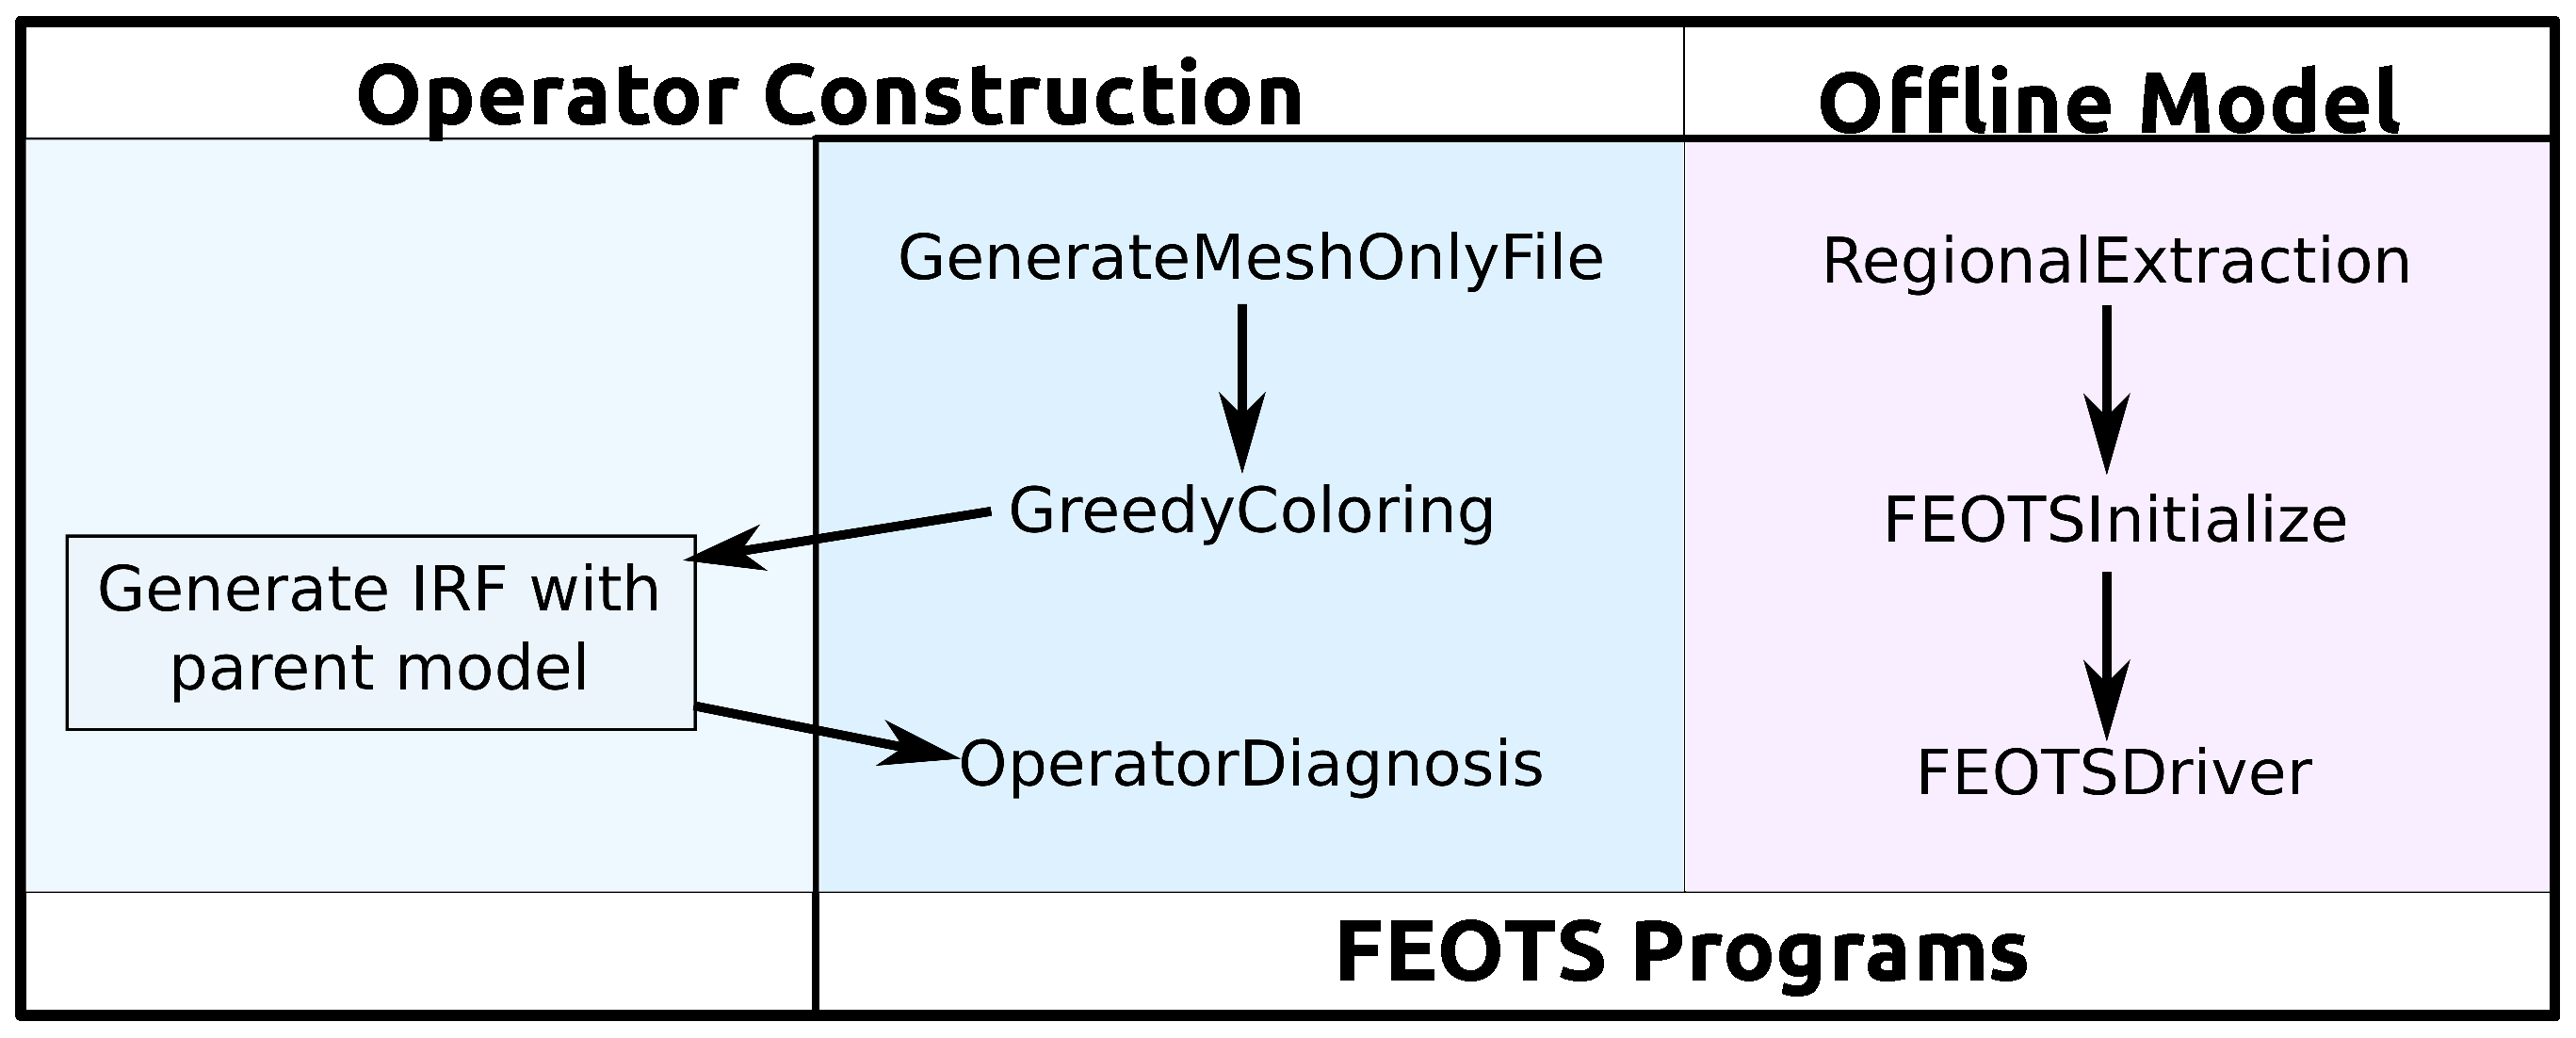
\includegraphics[width=0.95\textwidth]{workflow.eps}
\caption{A schematic depicting the two-stage workflow of operator construction followed by the offline tracer model. To accomplish this workflow, FEOTS provides six programs for each step. The order of execution is indicated by the arrows. Prior to running the offline model, a database of transport operators must be diagnosed from a parent model. }\label{fig:workflow}
\end{center}
\end{figure}


FEOTS views the workflow for running an offline tracer model in two stages 
\begin{enumerate}
\item Transport Operator Construction

\item Running the Offline Model
\end{enumerate}

For each stage, FEOTS provides three programs that divide the workflow into incremental steps. This division of steps is purposeful and is meant to provide stopping points for the user to check for any mistakes before proceeding through the workflow.

\section{Transport Operator Construction}

Transport operator construction is a process that diagnoses sparse matrices that are associated with advection and diffusion, consistent with a parent models formulation. In this process, a set of impulse fields are generated and should be passed through a parent models advection and diffusion routines. The impulse fields are generated by solving a graph coloring problem.  Using the impulse and impulse response fields, the sparse matrix representative of the transport operator can be diagnosed.



The graph is determined by the sparsity pattern of the advection-diffusion operators of the parent model. Currently, FEOTS has support for the Parallel Ocean Program (POP) with a tripole grid and Lax-Wendroff advection operators. If you're interested in using a  dipole grid and/or other advection schemes, contact Joe Schoonover (\textcolor{blue}{schoonover.numerics@gmail.com}). There are plans in place to offer support for transport operator construction in the MITgcm
\subsection{GenerateMeshOnlyFile}
This program will take a netcdf file, output by POP, extract only the mesh information and write a the mesh to a netcdf file with an additional ``mask'' field needed for the GreedyColoring.

\subsection{GreedyColoring}
Generates the impulse fields given a mesh and a stencil name. Currently, only the Lax Wendroff stencil is included. The impulse fields are then written to a netcdf file for use in POP. Additionally, the adjacency graph and its coloring are written to a binary file for later use.

\subsection{IRF Generation}
\subsubsection{ POP }

\subsection{OperatorDiagnosis}
Uses the Adjacency graph and its coloring (generated by GreedyColoring) in addition to impulse response fields to extract the sparse matrix representation of the transport operators. Before calling this program, GreedyColoring must be called to generate impulse fields, and the impulse fields need to be passed through POP to generate the impulse response fields 



\section{Running the Offline Model}

The offline FEOTS model can be run using the ``global'' transport operators or ``regional'' transport operators. Additionally, FEOTS has a package for tagging water masses based on locations and ocean state variables such as potential temperature, salinity, or potential density. When running in regional mode, a database of regional operators need to be extracted from the global operators
\subsection{GenMask}
This program can be used to generate a mask for picking out a domain for a regional simulation. It is likely that you will need to get a copy of the source code ( \texttt{src/POP/programs/GenMask.f90} ) and modify it to suit your particular application. This source code can be placed in any example directory that you create.

\subsection{RegionalExtraction}
Given latitudinal and longitudinal boundaries, this program constructs a data structure that maps between the global mesh and a regional mesh. Masks and mappings are constructed that are used to extract the appropriate rows and columns of the sparse transport matrices. These mappings are written to a binary file for later usage. A regional POP mesh is constructed and a “tracermask” field is filled in to indicate boundary cells; the regional POP mesh is written to a netcdf file for user inspection. Care was taken to ensure a correct mapping occurs for regions that cross the prime-meridian. Currently the regional extraction tool has not been tested on regions around the tripole centers.

\section{ExtractOceanState}

\section{FEOTSInitialize}
This program is used to set the initial conditions, source terms, relaxation time scales, additional masks, and “hard-set” values for the tracer fields. The initial fields and other terms are written to a netcdf file (Tracer.init.nc) for user inspection, to verify the configuration before beginning the actual run.

\section{FEOTSDriver}
The driver program manages the call to the “forward integrator” or the “equilibration” routines, and handles file I/O. This portion is currently in testing right now

\chapter{Configuring and Running FEOTS Programs}

\section{Software Acceleration with OpenMP}
If you have access to multicore architectures and a Fortran compiler with OpenMP support, the \texttt{FEOTSDriver} can be accelerated by enabling OpenMP. To build an OpenMP accelerated binary for the \texttt{FEOTSDriver}, set the environment variable \texttt{OMP} to \texttt{yes}. In a bash shell,
\begin{verbatim}
export OMP=yes
\end{verbatim} 
and in tcsh
\begin{verbatim}
setenv OMP yes
\end{verbatim}
With this variable set, executing
\begin{verbatim}
make FEOTSDriver
\end{verbatim}
from an example directory will enable OpenMP accelerations during compilation. Before running the executable, you must set the environment variable \texttt{OMP\_NUM\_THREADS} to the desired number of threads.\\

-- \textit{ provide scaling analysis on a few architectures and with a few additional openmp thread affinity options } ---

\section{Software Acceleration MPI}
If you have access to multicore architectures or a small computing cluster and a compiler with MPI capabilities, MPI can be used to parallelize FEOTS. It shoud be noted that currently, MPI is only function with the Passive Dye tracer and Settling Particulate models. The MPI implementation parallelizes the FEOTS routines by assigning each MPI rank to a single tracer and is only useful if you have multiple tracers. This is particularly useful for water-mass tagging problems over multiple boundaries, where the number of tracers can grow quickly. 

To build the MPI flavor of the \texttt{FEOTSDriver}, set the environment variable \texttt{MPI} to \texttt{yes}. In a bash shell,
\begin{verbatim}
export MPI=yes
\end{verbatim} 
and in tcsh
\begin{verbatim}
setenv MPI yes
\end{verbatim}
With this variable set, executing
\begin{verbatim}
make FEOTSDriver
\end{verbatim}
from an example directory should compile the FEOTSDriver using an MPI capable compiler. If your compiler is not in your default search path, you will need to modify a section of the makefile (\texttt{FEOTS/build/makefile}), so that the variable \texttt{FC} points to the correct compiler.
\begin{verbatim}
ifeq (${MPI},yes)
   FC=mpif90
   OPT+=-DHAVE_MPI
endif
\end{verbatim}

To run the FEOTSDriver with MPI, you must specify the number of processes to be the number of tracers plus one. This configuration is required since the master rank (rank 0) manages file I/O, while the other ranks handle computations. An incorrect configuration will cause the FEOTSDriver to stop within the initialization phase. As an example, if \texttt{nTracers=3} (and water mass tagging is turned off), then
\begin{verbatim}
   mpirun -np 4 ./FEOTSDriver
\end{verbatim}
would be the correct configuration. If water mass tagging is turned on, the number of tracers used is the number of masks multiplied by the number of layers.


\section{Hybrid MPI-OpenMP}
It is possible to run the \texttt{FEOTSDriver} with a hybrid MPI-OpenMP flavor. Before compilation, the environment variables \texttt{MPI} and \texttt{OMP} need to be set to \texttt{yes}. In a bash shell,
\begin{verbatim}
export MPI=yes
export OMP=yes
\end{verbatim} 
and in tcsh
\begin{verbatim}
setenv MPI yes
setenv OMP yes
\end{verbatim}
With this variable set, executing
\begin{verbatim}
make FEOTSDriver
\end{verbatim}
from an example directory should compile the \texttt{FEOTSDriver} using an MPI capable compiler with OpenMP enabled. Before running the executable, you must set the environment variable \texttt{OMP\_NUM\_THREADS} to the desired number of threads for each MPI rank.\\

The simplest method for executing the MPI-OpenMP flavor of the \texttt{FEOTSDriver} is to use (e.g.)
\begin{verbatim}
mpirun -np 4 -x OMP_NUM_THREADS ./FEOTSDriver
\end{verbatim}
It is likely that this encantation will not yield ideal performance for any given architecture. To obtain better performance, you will want to set the layout of the ranks and threads for the specific architecture you are running on.


\section{The Namelist File}

\subsection{POPMeshOptions} \label{sec:POPMeshOptions}

\begingroup\setlength{\fboxsep}{0pt}
  \colorbox{lightgray}{
    \begin{tabular}{p{0.25\linewidth} p{0.725\linewidth}}
    \toprule
    \textbf{MeshType} & \\
    \midrule
    \textbf{\textit{Type}} & \texttt{Character} \\
    \midrule
    \textbf{\textit{Description}} & Specifies the type of mesh used in the POP simulation. The mesh type is used to determine where periodic boundary conditions should be applied to aid in the construction of an adjacency graph and for performing regional mesh extraction. \\
    \midrule
    \textbf{\textit{Impacted Programs}} & \texttt{GreedyColoring}, \texttt{OperatorDiagnosis}, \texttt{RegionalExtraction} \\
    \midrule
    \textbf{\textit{Valid Options}}  & ``PeriodicTripole'' \\
    \bottomrule
\end{tabular}
}\endgroup

%\vspace{0.5cm}

\noindent\begingroup\setlength{\fboxsep}{0pt}
\colorbox{lightgray}{
\begin{tabular}{p{0.25\linewidth} p{0.725\linewidth}}
\toprule
\textbf{StencilType} & \\
\midrule
\textbf{\textit{Type}} & \texttt{Character} \\
\midrule
\textbf{\textit{Description}} & Specifies the advection stencil used in the POP simulation. The stencil type is used to determine cell connectivity when building an adjacency graph  \\
\midrule
\textbf{\textit{Impacted Programs}} & \texttt{GreedyColoring}, \texttt{OperatorDiagnosis}, \texttt{RegionalExtraction} \\
\midrule
\textbf{\textit{Valid Options}}  & ``LaxWendroff'' \\
\bottomrule
\end{tabular}
}\endgroup

%\vspace{0.5cm}

\noindent\begingroup\setlength{\fboxsep}{0pt}
\colorbox{lightgray}{
\begin{tabular}{p{0.25\linewidth} p{0.725\linewidth}}
\toprule
\textbf{Regional} & \\
\midrule
\textbf{\textit{Type}} & \texttt{Logical} \\
\midrule
\textbf{\textit{Description}} & A flag that specifies whether or not you are running a regional simulation. A regional domain, in FEOTS, is a domain that is a subset of the parent model. If Regional = .TRUE., you must also specify the bounding latitudes and longitudes. \\
\midrule
\textbf{\textit{Impacted Programs}} & \texttt{RegionalExtraction}, \texttt{FEOTSInitialize}, \texttt{FEOTSDriver} \\
\midrule
\textbf{\textit{Valid Options}}  & .TRUE. , .FALSE. \\
\bottomrule
\end{tabular}
}\endgroup

%\vspace{0.5cm}

\noindent\begingroup\setlength{\fboxsep}{0pt}
\colorbox{lightgray}{
\begin{tabular}{p{0.25\linewidth} p{0.725\linewidth}}
\toprule
\textbf{south} & \\
\midrule
\textbf{\textit{Type}} & \texttt{Real} \\
\midrule
\textbf{\textit{Description}} & Specifies the southern boundary of a regional domain in $^\circ$N. Negative values indicate latitudes in the southern hemisphere, positive values indicate latitudes in the northern hemisphere. \\
\midrule
\textbf{\textit{Impacted Programs}} & \texttt{RegionalExtraction} \\
\midrule
\textbf{\textit{Valid Options}}  & [-90.0,90.0], south $<$ north \\
\bottomrule
\end{tabular}
}\endgroup

%\vspace{0.5cm}

\noindent\begingroup\setlength{\fboxsep}{0pt}
\colorbox{lightgray}{
\begin{tabular}{p{0.25\linewidth} p{0.725\linewidth}}
\toprule
\textbf{north} & \\
\midrule
\textbf{\textit{Type}} & \texttt{Real} \\
\midrule
\textbf{\textit{Description}} & Specifies the northern boundary of a regional domain in $^\circ$N. Negative values indicate latitudes in the southern hemisphere, positive values indicate latitudes in the northern hemisphere. \\
\midrule
\textbf{\textit{Impacted Programs}} & \texttt{RegionalExtraction} \\
\midrule
\textbf{\textit{Valid Options}}  & [-90.0,90.0], north $>$ south \\
\bottomrule
\end{tabular}
}\endgroup

%\vspace{0.5cm}

\noindent\begingroup\setlength{\fboxsep}{0pt}
\colorbox{lightgray}{
\begin{tabular}{p{0.25\linewidth} p{0.725\linewidth}}
\toprule
\textbf{west} & \\
\midrule
\textbf{\textit{Type}} & \texttt{Real} \\
\midrule
\textbf{\textit{Description}} & Specifies the western boundary of a regional domain in $^\circ$E. Negative values indicate longitudes west of the prime-meridian, positive values indicate longitudes east of the prime-meridian. \\
\midrule
\textbf{\textit{Impacted Programs}} & \texttt{RegionalExtraction} \\
\midrule
\textbf{\textit{Valid Options}}  & [-360.0,360.0], west $<$ east \\
\bottomrule
\end{tabular}
}\endgroup

%\vspace{0.5cm}

\noindent\begingroup\setlength{\fboxsep}{0pt}
\colorbox{lightgray}{
\begin{tabular}{p{0.25\linewidth} p{0.725\linewidth}}
\toprule
\textbf{east} & \\
\midrule
\textbf{\textit{Type}} & \texttt{Real} \\
\midrule
\textbf{\textit{Description}} & Specifies the eastern boundary of a regional domain in $^\circ$E. Negative values indicate longitudes east of the prime-meridian, positive values indicate longitudes east of the prime-meridian. \\
\midrule
\textbf{\textit{Impacted Programs}} & \texttt{RegionalExtraction} \\
\midrule
\textbf{\textit{Valid Options}}  & [-360.0,360.0], east $>$ west \\
\bottomrule
\end{tabular}
}\endgroup

\noindent\begingroup\setlength{\fboxsep}{0pt}
\colorbox{lightgray}{
\begin{tabular}{p{0.25\linewidth} p{0.725\linewidth}}
\toprule
\textbf{MaskFile} & \\
\midrule
\textbf{\textit{Type}} & \texttt{Character} \\
\midrule
\textbf{\textit{Description}} & Specifies the NetCDF file to read and write a regional mask for selecting the regional domain. When \texttt{Regional} is set to \texttt{.FALSE.} this option is ignored. When the \texttt{MaskFile} is set, the latitude and longitude bounds are ignored  \\
\midrule
\textbf{\textit{Impacted Programs}} & \texttt{GenMask}, \texttt{RegionalExtraction}, \texttt{FEOTSInitialize}, \texttt{FEOTSDriver} \\
\midrule
\textbf{\textit{Valid Options}}  & ``LaxWendroff'' \\
\bottomrule
\end{tabular}
}\endgroup

\subsection{TracerModelOptions}

\noindent\begingroup\setlength{\fboxsep}{0pt}
\colorbox{lightgray}{
\begin{tabular}{p{0.25\linewidth} p{0.725\linewidth}}
\toprule
\textbf{TracerModel} & \\
\midrule
\textbf{\textit{Type}} & \texttt{Character} \\
\midrule
\textbf{\textit{Description}} & Specifies the type of passive tracer model to use. This influences the conditional evaluation in \texttt{src/solutionstorage/TracerStorage\_Class.f90}, subroutine \texttt{CalculateTendency\_TracerStorage}. If the Radionuclide Model or Settling Model are used, the settling velocity needs to be set. \\
\midrule
\textbf{\textit{Impacted Programs}} & \texttt{FEOTSInitialize}, \texttt{FEOTSDriver} \\
\midrule
\textbf{\textit{Valid Options}}  & ``DyeModel'', ``RadionuclideModel'', ``SettlingModel'' \\
\bottomrule
\end{tabular}
}\endgroup

\noindent\begingroup\setlength{\fboxsep}{0pt}
\colorbox{lightgray}{
\begin{tabular}{p{0.25\linewidth} p{0.725\linewidth}}
\toprule
\textbf{WaterMassTagging} & \\
\midrule
\textbf{\textit{Type}} & \texttt{Logical} \\
\midrule
\textbf{\textit{Description}} & A flag that specifies whether or not you are using the water-mass tagging capabilities in the code. If this feature is turned on and you are running a regional configuration, you must generate a database of the ocean state (temperature, salinity, density) using the \texttt{ExtractOceanState} program. \\
\midrule
\textbf{\textit{Impacted Programs}} & \texttt{FEOTSInitialize}, \texttt{FEOTSDriver} \\
\midrule
\textbf{\textit{Valid Options}}  & .TRUE. , .FALSE. \\
\bottomrule
\end{tabular}
}\endgroup

\noindent\begingroup\setlength{\fboxsep}{0pt}
\colorbox{lightgray}{
\begin{tabular}{p{0.25\linewidth} p{0.725\linewidth}}
\toprule
\textbf{settlingVelocity} & \\
\midrule
\textbf{\textit{Type}} & \texttt{Real} (Double Precision)  \\
\midrule
\textbf{\textit{Description}} & If \texttt{TracerModel}=``RadionuclideModel'' or ``SettlingModel'', the settling velocity is the fixed vertical velocity used to generate the vertical settling operator. \\
\midrule
\textbf{\textit{Impacted Programs}} & \texttt{FEOTSInitialize}, \texttt{FEOTSDriver} \\
\midrule
\textbf{\textit{Valid Options}}  & ``DyeModel'', ``RadionuclideModel'', ``SettlingModel'', ``BuoyantTracers'' \\
\bottomrule
\end{tabular}
}\endgroup

%\vspace{0.5cm}

\noindent\begingroup\setlength{\fboxsep}{0pt}
\colorbox{lightgray}{
\begin{tabular}{p{0.25\linewidth} p{0.725\linewidth}}
\toprule
\textbf{nTracers} & \\
\midrule
\textbf{\textit{Type}} & \texttt{Integer} \\
\midrule
\textbf{\textit{Description}} & The number of tracers for the offline model. If \texttt{TracerModel}=``RadionuclideModel'', this setting is ignored; the Radionuclide model supports 1 particulate and 1 radionuclide (2 tracers). For any other model, this parameter dictates how many tracer fields you want to work with. \textit{Since FEOTS operates on a shared memory parallelism, care must be taken to ensure that you do not run out of physical memory.}  \\
\midrule
\textbf{\textit{Impacted Programs}} & \texttt{FEOTSInitialize}, \texttt{FEOTSDriver} \\
\midrule
\textbf{\textit{Valid Options}}  & $\geq$ 1 \\
\bottomrule
\end{tabular}
}\endgroup

%\vspace{0.5cm}

\noindent\begingroup\setlength{\fboxsep}{0pt}
\colorbox{lightgray}{
\begin{tabular}{p{0.25\linewidth} p{0.725\linewidth}}
\toprule
\textbf{runMode} & \\
\midrule
\textbf{\textit{Type}} & \texttt{Character} \\
\midrule
\textbf{\textit{Description}} & Indicates whether you are running in ``Forward'' mode, in which transient behaviors of the tracers are desired, or ``Equilibrium'' mode in which an equilibrium solution is sought.  \\
\midrule
\textbf{\textit{Impacted Programs}} & \texttt{FEOTSDriver} \\
\midrule
\textbf{\textit{Valid Options}}  & ``Forward'', ``Equilibrium'' \\
\bottomrule
\end{tabular}
}\endgroup

\noindent\begingroup\setlength{\fboxsep}{0pt}
\colorbox{lightgray}{
\begin{tabular}{p{0.25\linewidth} p{0.725\linewidth}}
\toprule
\textbf{timeStepScheme} & \\
\midrule
\textbf{\textit{Type}} & \texttt{Character} \\
\midrule
\textbf{\textit{Description}} & Specifies the explicit integration scheme for any of the tracer models. Can be set to implement 1$^{st}$ Order Forward Euler, 2$^{nd}$ Order Adams-Bashforth, or 3$^{rd}$ Order Adams Bashforth. \\
\midrule
\textbf{\textit{Impacted Programs}} & \texttt{FEOTSDriver} \\
\midrule
\textbf{\textit{Valid Options}}  & ``Euler'', ``AB2'', ``AB3'' \\
\bottomrule
\end{tabular}
}\endgroup


\noindent\begingroup\setlength{\fboxsep}{0pt}
\colorbox{lightgray}{
\begin{tabular}{p{0.25\linewidth} p{0.725\linewidth}}
\toprule
\textbf{dt} & \\
\midrule
\textbf{\textit{Type}} & \texttt{Real} (Double Precision) \\
\midrule
\textbf{\textit{Description}} & The time step size for any forward integration. Note that this also impacts the equilibrium mode.  \\
\midrule
\textbf{\textit{Impacted Programs}} &  \texttt{FEOTSDriver} \\
\midrule
\textbf{\textit{Valid Options}}  & $>$ 0.0 \\
\bottomrule
\end{tabular}
}\endgroup

%\vspace{0.5cm}

\noindent\begingroup\setlength{\fboxsep}{0pt}
\colorbox{lightgray}{
\begin{tabular}{p{0.25\linewidth} p{0.725\linewidth}}
\toprule
\textbf{nTimeSteps} & \\
\midrule
\textbf{\textit{Type}} & \texttt{Integer} \\
\midrule
\textbf{\textit{Description}} & The number of desired time steps for running the \texttt{FEOTSDriver} in Forward mode. In Equilibrium mode, this option is ignored.  \\
\midrule
\textbf{\textit{Impacted Programs}} & \texttt{FEOTSDriver} \\
\midrule
\textbf{\textit{Valid Options}}  & $>$ 0 \\
\bottomrule
\end{tabular}
}\endgroup

%\vspace{0.5cm}

\noindent\begingroup\setlength{\fboxsep}{0pt}
\colorbox{lightgray}{
\begin{tabular}{p{0.25\linewidth} p{0.725\linewidth}}
\toprule
\textbf{nStepsPerDump} & \\
\midrule
\textbf{\textit{Type}} & \texttt{Integer} \\
\midrule
\textbf{\textit{Description}} & In Forward mode, this is the number of time steps taken between each netcdf file output. In Equilibrium mode, this is the number of nonlinear iterations taken between each netcdf pickup file output. \\
\midrule
\textbf{\textit{Impacted Programs}} & \texttt{FEOTSDriver} \\
\midrule
\textbf{\textit{Valid Options}}  & $\geq$ 1 \\
\bottomrule
\end{tabular}
}\endgroup

\subsection{OperatorOptions}
\noindent\begingroup\setlength{\fboxsep}{0pt}
\colorbox{lightgray}{
\begin{tabular}{p{0.25\linewidth} p{0.725\linewidth}}
\toprule
\textbf{OperatorPeriod} & \\
\midrule
\textbf{\textit{Type}} & \texttt{Real} (Double Precision) \\
\midrule
\textbf{\textit{Description}} & The length of time (in seconds) for which each transport operator should be applied. \\
\midrule
\textbf{\textit{Impacted Programs}} & \texttt{FEOTSDriver} \\
\midrule
\textbf{\textit{Valid Options}}  & $>$ 0.0 \\
\bottomrule
\end{tabular}
}\endgroup

%\vspace{0.5cm}

\noindent\begingroup\setlength{\fboxsep}{0pt}
\colorbox{lightgray}{
\begin{tabular}{p{0.25\linewidth} p{0.725\linewidth}}
\toprule
\textbf{nOperatorsPerCycle} & \\
\midrule
\textbf{\textit{Type}} & \texttt{Integer} \\
\midrule
\textbf{\textit{Description}} & The number of transport operators to cycle over before repeating. \textit{Ex.:} If nOperatorsPerCycle=5, FEOTS will use the first five transport operators and continue integration by repeating over these operators. \\
\midrule
\textbf{\textit{Impacted Programs}} & \texttt{FEOTSDriver} \\
\midrule
\textbf{\textit{Valid Options}}  & $\geq$ 1 \\
\bottomrule
\end{tabular}
}\endgroup

\subsection{FileOptions}\label{sec:FileOptions}
\noindent\begingroup\setlength{\fboxsep}{0pt}
\colorbox{lightgray}{
\begin{tabular}{p{0.25\linewidth} p{0.725\linewidth}}
\toprule
\textbf{extractRegionalOperators} & \\
\midrule
\textbf{\textit{Type}} & \texttt{Logical} \\
\midrule
\textbf{\textit{Description}} & A flag used to indicate whether regional operators should be extracted. If set to .FALSE., the \texttt{RegionalExtraction} program will only generate a regional mesh and the local-to-global mapping. If set to .TRUE., the \texttt{RegionalExtraction} program will also diagnose regional transport operators. \\
\midrule
\textbf{\textit{Impacted Programs}} & \texttt{RegionalExtraction} \\
\midrule
\textbf{\textit{Valid Options}}  & \texttt{.TRUE.}, \texttt{.FALSE.} \\
\bottomrule
\end{tabular}
}\endgroup

%\vspace{0.5cm}

\noindent\begingroup\setlength{\fboxsep}{0pt}
\colorbox{lightgray}{
\begin{tabular}{p{0.25\linewidth} p{0.725\linewidth}}
\toprule
\textbf{graphFile} & \\
\midrule
\textbf{\textit{Type}} & \texttt{Character} \\
\midrule
\textbf{\textit{Description}} & Specifies the file where the FEOTS Adjacency graph is stored for a particular parent model.  \\
\midrule
\textbf{\textit{Impacted Programs}} & \texttt{GreedyColoring}, \texttt{DiagnoseOperators}, \texttt{RegionalExtraction} \\
\midrule
\textbf{\textit{Valid Options}}  & File name with path less than or equal to 400 characters. \\
\bottomrule
\end{tabular}
}\endgroup

\noindent\begingroup\setlength{\fboxsep}{0pt}
\colorbox{lightgray}{
\begin{tabular}{p{0.25\linewidth} p{0.725\linewidth}}
\toprule
\textbf{IRFListFile} & \\
\midrule
\textbf{\textit{Type}} & \texttt{Character} \\
\midrule
\textbf{\textit{Description}} & Specifies the file that contains a list of all of the Impulse Response Function NetCDF files generated by the parent model. \textit{Ex :} If the environment variable \texttt{IRFDIR} defines the path to the IRF files, this file can be generated with the command \texttt{ ls \$IRFDIR > IRFfiles.txt }. Then, in the namelist file (\texttt{runtime.params}), \texttt{IRFListFile = IRFfiles.txt,} . \\
\midrule
\textbf{\textit{Impacted Programs}} & \texttt{DiagnoseOperators}, \texttt{RegionalExtraction} \\
\midrule
\textbf{\textit{Valid Options}}  & File name with path less than or equal to 400 characters. \\
\bottomrule
\end{tabular}
}\endgroup

\noindent\begingroup\setlength{\fboxsep}{0pt}
\colorbox{lightgray}{
\begin{tabular}{p{0.25\linewidth} p{0.725\linewidth}}
\toprule
\textbf{IRFStart} & \\
\midrule
\textbf{\textit{Type}} & \texttt{Integer} \\
\midrule
\textbf{\textit{Description}} & Specifies the file that contains a list of all of the Impulse Response Function NetCDF files generated by the parent model. \textit{Ex :} If the environment variable \texttt{IRFDIR} defines the path to the IRF files, this file can be generated with the command \texttt{ ls \$IRFDIR > IRFfiles.txt }. Then, in the namelist file (\texttt{runtime.params}), \texttt{IRFListFile = IRFfiles.txt,} . \\
\midrule
\textbf{\textit{Impacted Programs}} & \texttt{DiagnoseOperators}, \texttt{RegionalExtraction} \\
\midrule
\textbf{\textit{Valid Options}}  & 0 $<$ \texttt{IRFStart} $\leq$ \texttt{nIRFFiles}  \\
\bottomrule
\end{tabular}
}\endgroup

\noindent\begingroup\setlength{\fboxsep}{0pt}
\colorbox{lightgray}{
\begin{tabular}{p{0.25\linewidth} p{0.725\linewidth}}
\toprule
\textbf{nIRFFiles} & \\
\midrule
\textbf{\textit{Type}} & \texttt{Integer} \\
\midrule
\textbf{\textit{Description}} & The number of Impulse Response Function NetCDF files generated by the parent model. \textit{Ex :} If the environment variable \texttt{IRFFiles.txt} is set as the \texttt{IRFListFile} and the number of IRF files is not known a'priori, the command \texttt{wc -l IRFFiles.txt} will return the number of IRF files. \\
\midrule
\textbf{\textit{Impacted Programs}} & \texttt{DiagnoseOperators}, \texttt{RegionalExtraction} \\
\midrule
\textbf{\textit{Valid Options}}  &  $>$ 0 \\
\bottomrule
\end{tabular}
}\endgroup

\noindent\begingroup\setlength{\fboxsep}{0pt}
\colorbox{lightgray}{
\begin{tabular}{p{0.25\linewidth} p{0.725\linewidth}}
\toprule
\textbf{feotsOperatorDirectory} & \\
\midrule
\textbf{\textit{Type}} & \texttt{Character} \\
\midrule
\textbf{\textit{Description}} & Specifies the directory where the transport operators for a given parent model should be stored or read from. \\
\midrule
\textbf{\textit{Impacted Programs}} & \texttt{DiagnoseOperators}, \texttt{RegionalExtraction}, \texttt{FEOTSDriver} \\
\midrule
\textbf{\textit{Valid Options}}  & File name with path less than or equal to 400 characters. \\
\bottomrule
\end{tabular}
}\endgroup

\noindent\begingroup\setlength{\fboxsep}{0pt}
\colorbox{lightgray}{
\begin{tabular}{p{0.25\linewidth} p{0.725\linewidth}}
\toprule
\textbf{regionalOperatorDirectory} & \\
\midrule
\textbf{\textit{Type}} & \texttt{Character} \\
\midrule
\textbf{\textit{Description}} & Specifies the directory where a set of regional transport operators should be stored or read from. \\
\midrule
\textbf{\textit{Impacted Programs}} & \texttt{RegionalExtraction}, \texttt{FEOTSDriver} \\
\midrule
\textbf{\textit{Valid Options}}  & File name with path less than or equal to 400 characters. \\
\bottomrule
\end{tabular}
}\endgroup

\noindent\begingroup\setlength{\fboxsep}{0pt}
\colorbox{lightgray}{
\begin{tabular}{p{0.25\linewidth} p{0.725\linewidth}}
\toprule
\textbf{operatorBaseName} & \\
\midrule
\textbf{\textit{Type}} & \texttt{Character} \\
\midrule
\textbf{\textit{Description}} & When the transport operators are written to file, a connectivity (.conn) and data (.data) file are written for advection and difussion operators with the same ``base-name''. \texttt{operatorBaseName} determines this base name. \textit{Ex :} If \texttt{operatorBaseName = pop\_03\_tripole,} then the transport operator files will be written in files \texttt{pop\_03\_tripole\_advect.NNNNN.data}, \texttt{pop\_03\_tripole\_advect.NNNNN.conn}, \texttt{pop\_03\_tripole\_diffu.NNNNN.data} , and \texttt{pop\_03\_tripole\_diffu.NNNNN.conn}, where the \texttt{NNNNN} is an integer padded with zeros indicating which operator it corresponds to.  \\
\midrule
\textbf{\textit{Impacted Programs}} & \texttt{DiagnoseOperators}, \texttt{RegionalExtraction}, \texttt{FEOTSDriver} \\
\midrule
\textbf{\textit{Valid Options}}  & String less than or equal to 100 characters. \\
\bottomrule
\end{tabular}
}\endgroup

\noindent\begingroup\setlength{\fboxsep}{0pt}
\colorbox{lightgray}{
\begin{tabular}{p{0.25\linewidth} p{0.725\linewidth}}
\toprule
\textbf{meshFile} & \\
\midrule
\textbf{\textit{Type}} & \texttt{Character} \\
\midrule
\textbf{\textit{Description}} & Specifies the NetCDF file that stores the POP Mesh information associated with the full parent model in addition to a mask generated from the KMT field.  \\
\midrule
\textbf{\textit{Impacted Programs}} & \texttt{GenerateMeshOnlyFile}, \texttt{DiagnoseOperators}, \texttt{RegionalExtraction}, \texttt{FEOTSInitialize}, \texttt{FEOTSDriver} \\
\midrule
\textbf{\textit{Valid Options}}  & File name with path less than or equal to 400 characters. \\
\bottomrule
\end{tabular}
}\endgroup

\noindent\begingroup\setlength{\fboxsep}{0pt}
\colorbox{lightgray}{
\begin{tabular}{p{0.25\linewidth} p{0.725\linewidth}}
\toprule
\textbf{regionalMeshFile} & \\
\midrule
\textbf{\textit{Type}} & \texttt{Character} \\
\midrule
\textbf{\textit{Description}} & Specifies the NetCDF file that stores a regional mesh with its mask for a given parent model and regional configuration. \\
\midrule
\textbf{\textit{Impacted Programs}} & \texttt{RegionalExtraction}, \texttt{FEOTSInitialize}, \texttt{FEOTSDriver} \\
\midrule
\textbf{\textit{Valid Options}}  & File name with path less than or equal to 400 characters. \\
\bottomrule
\end{tabular}
}\endgroup

\subsection{JFNKOptions}

\noindent\begingroup\setlength{\fboxsep}{0pt}
\colorbox{lightgray}{
\begin{tabular}{p{0.25\linewidth} p{0.725\linewidth}}
\toprule
\textbf{maxItersJFNK} & \\
\midrule
\textbf{\textit{Type}} & \texttt{Integer} \\
\midrule
\textbf{\textit{Description}} & Specifies the maximum number of outer, nonlinear, iterations for the ``Newton part'' of the JFNK solver. \\
\midrule
\textbf{\textit{Impacted Programs}} & \texttt{FEOTSDriver} \\
\midrule
\textbf{\textit{Valid Options}}  & $>$ 0\\
\bottomrule
\end{tabular}
}\endgroup

\noindent\begingroup\setlength{\fboxsep}{0pt}
\colorbox{lightgray}{
\begin{tabular}{p{0.25\linewidth} p{0.725\linewidth}}
\toprule
\textbf{toleranceJFNK} & \\
\midrule
\textbf{\textit{Type}} & \texttt{Real} (Double Precision) \\
\midrule
\textbf{\textit{Description}} & The error tolerance (stop criteria) for the nonlinear solver. \\
\midrule
\textbf{\textit{Impacted Programs}} & \texttt{FEOTSDriver} \\
\midrule
\textbf{\textit{Valid Options}}  & $>$ 0.0 , \textit{Default :} $10^{-7}$\\
\bottomrule
\end{tabular}
}\endgroup

\noindent\begingroup\setlength{\fboxsep}{0pt}
\colorbox{lightgray}{
\begin{tabular}{p{0.25\linewidth} p{0.725\linewidth}}
\toprule
\textbf{maxItersGMRES} & \\
\midrule
\textbf{\textit{Type}} & \texttt{Integer} \\
\midrule
\textbf{\textit{Description}} & Specifies the maximum number of restarts for the GMRES-with-restarts inner, linear, solver; the ``Krylov'' part of the JNFK solver. \\
\midrule
\textbf{\textit{Impacted Programs}} & \texttt{FEOTSDriver} \\
\midrule
\textbf{\textit{Valid Options}}  & $>$ 0\\
\bottomrule
\end{tabular}
}\endgroup

\noindent\begingroup\setlength{\fboxsep}{0pt}
\colorbox{lightgray}{
\begin{tabular}{p{0.25\linewidth} p{0.725\linewidth}}
\toprule
\textbf{mInnerItersGMRES} & \\
\midrule
\textbf{\textit{Type}} & \texttt{Integer} \\
\midrule
\textbf{\textit{Description}} & Specifies the size of the Krylov subspace to search for a solution on the inner iterates of the GMRES solver. \\
\midrule
\textbf{\textit{Impacted Programs}} & \texttt{FEOTSDriver} \\
\midrule
\textbf{\textit{Valid Options}}  & $>$ 0\\
\bottomrule
\end{tabular}
}\endgroup

\noindent\begingroup\setlength{\fboxsep}{0pt}
\colorbox{lightgray}{
\begin{tabular}{p{0.25\linewidth} p{0.725\linewidth}}
\toprule
\textbf{toleranceGMRES} & \\
\midrule
\textbf{\textit{Type}} & \texttt{Real} (Double Precision) \\
\midrule
\textbf{\textit{Description}} & The error tolerance (stop criteria) for the GMRES linear solver. \\
\midrule
\textbf{\textit{Impacted Programs}} & \texttt{FEOTSDriver} \\
\midrule
\textbf{\textit{Valid Options}}  & $>$ 0.0 , \textit{Default :} $10^{-7}$\\
\bottomrule
\end{tabular}
}\endgroup


\noindent\begingroup\setlength{\fboxsep}{0pt}
\colorbox{lightgray}{
\begin{tabular}{p{0.25\linewidth} p{0.725\linewidth}}
\toprule
\textbf{JacobianStepSize} & \\
\midrule
\textbf{\textit{Type}} & \texttt{Real} (Double Precision) \\
\midrule
\textbf{\textit{Description}} & The step size for approximating the Jacobian matrix action. \\
\midrule
\textbf{\textit{Impacted Programs}} & \texttt{FEOTSDriver} \\
\midrule
\textbf{\textit{Valid Options}}  & $>$ 0.0, \textit{Default :} $10^{-2}$\\
\bottomrule
\end{tabular}
}\endgroup

\noindent\begingroup\setlength{\fboxsep}{0pt}
\colorbox{lightgray}{
\begin{tabular}{p{0.25\linewidth} p{0.725\linewidth}}
\toprule
\textbf{isPickupRun} & \\
\midrule
\textbf{\textit{Type}} & \texttt{Logical} \\
\midrule
\textbf{\textit{Description}} & Indicates whether the equilibration run is a pickup run. If set to \texttt{.TRUE.}, the \texttt{FEOTSDriver} will attempt to open a file \texttt{Tracer.pickup.nc} as the initial condition. If set to \texttt{.FALSE.}, the \texttt{FEOTSDriver} will attempt to open a file \texttt{Tracer.init.nc} as the initial condition. \\
\midrule
\textbf{\textit{Impacted Programs}} & \texttt{FEOTSDriver} \\
\midrule
\textbf{\textit{Valid Options}}  & \texttt{.TRUE.}, \texttt{.FALSE.} \\
\bottomrule
\end{tabular}
}\endgroup


\section{Setting up your own example}
 When developing your own example problem for the offline tracer model, it is easiest to copy an existing example that is most similar to your desired setup, and make modifications from there. In any situation, you will want to copy the following files from a pre-configured example :
 
 \vspace{0.5cm}
 \begin{flushleft}
\begingroup\setlength{\fboxsep}{0pt}
  \colorbox{lightgray}{
    \begin{tabular}{p{0.25\linewidth} | p{0.725\linewidth}}
    \toprule
    \texttt{FEOTSInitialize.f90} & Fortran source code for setting up the initial conditions, source terms, masks, and hard-set tracer values.\\
    \midrule
    \texttt{GenMask.f90} & An optional Fortran source code for generating a regional mask.\\
    \midrule
    \texttt{makefile} & A local makefile that manages calls to the master makefile and assures compilation of the local FEOTSInitialize.f90 source code for the FEOTSInitialize program. \\
    \midrule
    \texttt{runtime.params} & Namelist file for configuring your model simulation\\
    \bottomrule
\end{tabular}
}\endgroup
\end{flushleft}
\vspace{0.5cm}

\subsection{Generating Impulse Fields for IRF Generation}
\textit{\textbf{Disclaimer} : Currently, FEOTS is only setup for working with the POP Tripole Grid and the Lax-Wendroff advection scheme (7 point stencil). However, adding other grids and advection schemes is quite easy. Contact \href{mailto:schoonover.numerics@gmail.com}{schoonover.numerics@gmail.com} about adding more functionality.} \\

 

\subsection{Setting your File I/O Options}

\subsection{Regional Simulation with Lat/Lon Bounds}
Regional domains and transport operators can be constructed using one of two strategies :
\begin{enumerate}
\item Specifying latitude and longitude boundaries
\item Providing a mask in a NetCDF file
\end{enumerate} 
In either approach, the \texttt{Regional} parameter underneath the \texttt{POPMeshOptions} namelist must be set to \texttt{.TRUE.} .

 The simplest method for performing a regional simulation is to specify the latitude and longitude boundaries using the \texttt{south}, \texttt{north}, \texttt{west}, and \texttt{east} parameters. In this case, the \texttt{POPMeshOptions} namelist within the \texttt{runtime.params} namelist file would look similar to the example given below
\begin{verbatim}
&POPMeshOptions
Regional = .TRUE.,
south    = -60.0,
north    = -20.0,
west     = -10.0,
east     = -20.0,
/
\end{verbatim}
With this configuration, in addition to the File Options being configured properly, you can compile and run the \texttt{RegionalExtraction} program to generate the necessary files for performing a regional experiment. By default, this program will generate a NetCDF file that contains the regional mesh and will subsample all of the transport operators. If you need to fine-tune the regional extraction and temporarily avoid extracting all of the operators, you can set the \texttt{extractRegionalOperators} parameter to \texttt{.FALSE.} under the \texttt{FileOptions} namelist. In this mode, the \texttt{RegionalExtraction} program will only create the NetCDF file corresponding to the name provided in the \texttt{regionalMeshFile} parameter.

\subsection{Regional Simulation with a User-provided Mask}

\subsection{Initial Conditions}
Of these three files, only FEOTSInitialize.f90 and runtime.params need to be modified to design a new example, provided you have access to an existing set of transport operators. Within FEOTSInitialize.f90, there is one subroutine that can be modified to set up the initial tracer distribution and the source and mask terms  : \texttt{InitialConditions}

To explain how to assign the initial conditions, a brief overview of the \texttt{POP\_FEOTS} data structure is needed.
 
 

\subsection{Water Mass Tagging}
 \textit{\textbf{Disclaimer} : Currently, water mass tagging is configured to work only with regional experiments. Enabling water mass tagging on a global simulation has not been tested.}
 
The development of an experiment with water mass taggging begins at the \texttt{RegionalExtraction} stage of the FEOTS workflow. If your region is chosen without providing a region mask, then all of the boundary points by default are set as prescribed boundary points. This means that water mass tagging will occur at all boundary points. Alternatively, if you provide a region mask, setting grid points to -1 corresponds to that point being a prescribed point. When performing water mass tagging experiments, it is recommended that you supply a region mask as this provides you with the most control on where to prescribe tracer injections.

 
In addition to setting up the regional domain and performing regional operator extraction, you must compile and run the \texttt{ExtractOceanState} program to generate a database of NetCDF files that contain the temperature, salinity, and potential density output from POP for your region. Successful execution of the \texttt{ExtractOceanState} program should result in \texttt{Ocean.*.nc} files in the directory specified by \texttt{regionalOperatorDirectory} parameter in the \texttt{runtime.params} namelist file. At this point, you can run the \texttt{FEOTSInitialize} program.

Before running the \texttt{FEOTSDriver} program, there are a couple options in the namelist file that need to be set. Under the \texttt{TracerModelOptions} namelist, the \texttt{WaterMassTagging} parameter must be set to \texttt{.TRUE.} . It is recommended that the \texttt{TracerModel} is set to \texttt{"DyeModel"}. If you want to tag multiple water masses, set \texttt{nTracers} to the desired number. Keep in mind that increasing the number of tracers increases memory consumption and can increase wall-time. 

Last, you must create a file called \texttt{watermass.config}. The first line of this file should indicate the ocean state variable that you are using to tag water masses. Valid options include \texttt{Temperature}, \texttt{Salinity}, or \texttt{Density}. This option is not case sensitive, though incorrect spelling or any other invalid option will result in the \texttt{FEOTSDriver} stopping. The next few lines should list the lower and upper bounds of the ocean state variable for each tracer. For example, if the contents of \texttt{watermass.config} are
\begin{verbatim}
Temperature
5.0 10.0
10.0 15.0
15.0 20.0
\end{verbatim}
and \texttt{nTracers = 3,} in \texttt{runtime.params}, then for each operator the \texttt{FEOTSDriver} will hard set the first dye tracer to 1 where temperature values are between 5$^\circ$ C and 10$^\circ$ C and 0 at other prescribed points, the second dye tracer to 1 where temperature values are between 10$^\circ$ C and 15$^\circ$ C and 0 at other prescribed points, etc.

%\section{Adding a new tracer model}
 
\chapter{Examples} \label{chapter:examples}

\section{Parent Models}
\subsection{POP03T} \label{sec:POP03T}
\textit{Need documentation on the 0.3 degree POP Tripole configuration}

\section{Global Operator Diagnosis}\label{sec:GlobalOperatorDiagnosis}
\begin{center}
\texttt{FEOTS/examples/POP03T\_OperatorDiagnosis}
\end{center}
This example summarizes the procedure for diagnosing transport operators for use with the FEOTS Offline tracer models; it demonstrates the first stage of the FEOTS workflow.

\subsection{Generating the Impulse Fields}
In the first step towards generating the transport operators, the POP model should be configured and run for a single time step to produce a NetCDF file that contains the mesh of the parent model. In this example, the parent model is POP03T, which is described in Section \ref{sec:POP03T}. The contents of the \texttt{runtime.params} namelist file is shown here 
\begin{verbatim}
&POPMeshOptions
MeshType    = 'PeriodicTripole',
StencilType = 'LaxWendroff',
/
&TracerModelOptions
/
&OperatorOptions
/
&FileOptions
meshfile                  ='/usr/projects/cesm/FastSolver/feots/
                            database/POP_0.3_Operators_5DayAvg/POP_03deg_mesh.nc',
graphfile                 ='/usr/projects/cesm/FastSolver/feots/
                            database/POP_0.3_Operators_5DayAvg/
                            pop_03_periodic-tripole_laxwendroff',
operatorBaseName          = 'pop_03_periodic-tripole',
feotsOperatorDirectory    ='/usr/projects/cesm/FastSolver/feots/
                            database/POP_0.3_Operators_5DayAvg/Global/',
IRFListFile               = 'IRFList_5dayAvg.txt',
IRFStart                  = 1,
nIRFFiles                 = 365,
/
&JFNKOptions
/
\end{verbatim}

The \texttt{MeshType} is set to \texttt{PeriodicTripole} and the \texttt{StencilType} is set to LaxWendroff, consistent with the configuration of the POP03T parent model. The \texttt{FileOptions} namelist determines where the read the parent model mesh from, and where to write the adjacencey graph file and the transport operators. A description of each of the options in the namelist file are given in Sections \ref{sec:POPMeshOptions} and \ref{sec:FileOptions}.

To generate the impulse fields that will be passed to the POP model, the \texttt{GreedyColoring} program is used. Underneath the directory \texttt{FEOTS/examples/POP03T\_OperatorDiagnosis}, run
\begin{verbatim}
make GreedyColoring
\end{verbatim}
This compiles source code for generating the executable for generating the Impulse Fields. This program is run by executing
\begin{verbatim}
./GreedyColoring
\end{verbatim}
The output from running this program for the POP03T parent model is shown in Figure



\pagebreak
\section{Agulhas Regional Operator Diagnosis and Passive Dye Injection}
\begin{center}
\texttt{FEOTS/examples/agulhas}
\end{center}
\begin{figure}[t!]
\centering
\includegraphics[width=0.75\linewidth,natwidth=600,natheight=549]{agulhas_local_sourcespot.png}
\caption{This image shows the dye source on the southeast coast of Africa...}\label{fig:agulhasSource}
\end{figure}
In this example, the equation
\begin{equation}
 c_t + \vec{u} \cdot \nabla c = r( c_f - c )
\end{equation}
is solved, where $c$ is the concentration of a passive ``dye'' tracer, $\vec{u}$ is the velocity field, $c_f$ is a relaxation field, and $r$ is a spatially dependent relaxation frequency. For this example, the relaxation field and frequency are specified as a Gaussian in latitude and longitude and independent of the vertical coordinate $z$,
\begin{subequations}
\begin{align}
  c_f &= c_0 \\
  r   &= r_0 e^{ -\left( \frac{ (x-x_0)^2 + (y-y_0)^2 }{2 L^2 }\right)}
\end{align}
\end{subequations}
where the parameters $c_0$, $r_0$, $x_0$, $y_0$, and $L$ are shown in Table \ref{table:agulhasSourceParameters} and the dye source field at the surface layer is shown in Figure \ref{fig:agulhasSource}.
\begin{table}
\caption{} \label{table:agulhasSourceParameters}
\begin{center}
\begin{tabular}{ | c | c |}
\hline
$c_0$ & $5.0$ \\
\hline
$r_0$ & $2.31 \times 10^{-5}$ s$^{-1}$\\
\hline
$x_0$ & $31.5^\circ E$\\
\hline
$y_0$ & $31.0^\circ S$\\
\hline
$L$ & $0.354^\circ$ \\
\hline
\end{tabular}
\end{center}
\end{table}

The advection is modeled using one year repeat cycles of the 5-day averaged transport operators diagnosed from the POP03T parent model; the advection operator is diagnosed from the 2nd order Lax Wendroff advection scheme. 

\subsection{Configuration}
The setup for this model can be described by the contents of the \texttt{runtime.params} namelist file. Here, the impact of each option in the namelists are explained. The first namelist is \texttt{POPMeshOptions} and is shown below.

\begin{verbatim}
&POPMeshOptions
MeshType    = 'PeriodicTripole',
StencilType = 'LaxWendroff',
Regional    = .TRUE.,
south       = -60.0,
east        = 50.0,
west        = -10.0,
north       = -20.0,  
/
\end{verbatim}
The mesh-type is specified as a periodic tripole mesh, to correspond to the type of mesh that is used in the POP03T parent model. The stencil-type is specifies that the advection scheme is the second order Lax-Wendroff. These options only influence the \texttt{GreedyColoring} and the \texttt{OperatorDiagnosis} programs; they do not influence the initialization and driver programs.

The ``Regional'' flag is set to \texttt{.TRUE.} to indicate that we are running a regional simulation, and the latitudinal and longitudinal boundaries are set encompass the southern tip of Africa and the Agulhas retroflection. When a regional simulation is desired, it is necessary to run the \texttt{RegionalExtraction} program first in order to build a database of transport operators for the specified region.

\subsection{Regional Operator Extraction}
When extracting regional operators, you must have global operators already diagnosed from the parent model. The \texttt{FileOptions} namelist is used to set up the necessary parameters for the \texttt{RegionalExtraction} program. Here, the relevant options are shown and discussed
\begin{verbatim}
&FileOptions
extractRegionalOperators  = .TRUE.,
meshfile                  ='/usr/projects/cesm/FastSolver/feots/database/
                            POP_0.3_Operators_5DayAvg/POP_03deg_mesh.nc',
regionalmeshfile          ='Agulhas_mesh.nc', 
graphfile                 ='/usr/projects/cesm/FastSolver/feots/database/
                            POP_0.3_Operators_5DayAvg/
                            pop_03_periodic-tripole_laxwendroff',
operatorBaseName          = 'pop_03_periodic-tripole',
feotsOperatorDirectory    ='/usr/projects/cesm/FastSolver/feots/database/
                            POP_0.3_Operators_5DayAvg/Global/',
regionalOperatorDirectory ='/usr/projects/cesm/FastSolver/feots/database/
                            POP_0.3_Operators_5DayAvg/Agulhas/',
/
\end{verbatim}
The \texttt{extractRegionalOperators} flag is set to \texttt{.TRUE.} to indicate that we want to extract regional operators. The \texttt{meshfile} points to the location of a NetCDF containing the global mesh for the parent model. The \texttt{regionalmeshfile} points to the desired location to write out the regional mesh after it has been extracted from the global mesh. The \texttt{graphfile} points to the location of the FEOTS generated graph-file associated with parent model's global mesh and advection scheme; this was generated with the \texttt{GreedyColoring} program. \texttt{feotsOperatorDirectory} points to the directory that contains the global transport operators and \texttt{regionalOperatorDirectory} points to a directory where you will write the regional operators to hard disk. 

To build the RegionalExtraction executable, run
\begin{verbatim}
make RegionalExtraction
\end{verbatim}
Then, to run this executable
\begin{verbatim}
./RegionalExtration
\end{verbatim}

\subsection{Running the Model}
After the regional operators have been extracted, the namelists \texttt{TracerModelOptions} and \texttt{OperatorOptions} must be set up to run the initialization and driver programs. The settings for these namelists are shown here :
\begin{verbatim}
&TracerModelOptions
TracerModel = 'DyeModel',
dt          = 1080.0,
runMode     = 'Forward',
nStepsPerDump   = 80,
iterInit        = 0,
nTimeSteps      = 160,
/
&OperatorOptions
operatorPeriod = 432000.0,
nOperatorsPerCycle = 73,
/
\end{verbatim}
In the \texttt{TracerModelOptions}, it is indicated that the tracer model is the Passive Dye Model. The simulation will proceed in Forward Mode, so that we can model the transient behavior of the dye spreading from the source. The integration uses a time step of 1080 seconds and every 80 time steps, an output file is written. Currently the configuration shows only 160 time steps to be done. The \texttt{OperatorOptions} indicate that each operator should be applied for intervals of 432,000 seconds (5 days) and we will use repeat cycles of 73 operators (1 year).

To run the model, initial conditions must first be generated. This is then followed by the driver program
\begin{verbatim}
make FEOTSInitialize FEOTSDriver
./FEOTSInitialize
./FEOTSDriver
\end{verbatim}

With the given configuration, this should generate four NetCDF files : Tracer.init.nc, Tracer.0000000000.nc, Tracer.0000000080.nc, Tracer.0000000160.nc.



\section{Global Particulate-Radionuclide}
%\section{Passive Micro-plastics}


\part{Technical Documentation}

\chapter{Introduction}

Biological and chemical tracers can be transported throughout the world's oceans through advection and diffusion processes. Additionally, these tracers can change their concentration/activity levels through coupled interactions that are often nonlinear. The time scale for equilibration of most oceanic passive\footnote{\textit{Passive, here, means that the tracer does not impact the momentum of mass balances of the fluid's governing equations}} tracers is on the order of hundreds to thousands of years. Global simulations of the ocean are now routinely being conducted at resolutions of 10 km and smaller, for which the explicit advective CFL limit yields a time step on the order of $\frac{1}{10}$ day. Online simulations, in which tracers are advected in tandem with forward integration of the fluid momentum equations, will typically have even more restrictive stability constraints due to the presence of other, faster modes in the momentum equations. Offline simulations do not suffer from the additional overhead associated with a full-blown GCM, though a tremendous hurdle remains in using the velocity and diffusivity fields in a manner consistent with GCM discretization and parameterizations. The Fast Equilibration of Ocean Tracers Software (FEOTS) offers the ability to overcome this hurdle by providing tools to 
\begin{enumerate}
  \item Aid in the diagnosis of advection and diffusion operators from online fluid simulations,     
  \item Perform offline forward integration of passive tracers, and 
  \item Rapidly equilibrate passive tracer systems through root-finding and minimization strategies.
\end{enumerate}

   FEOTS is inspired by the work of those before us, particularly \citet{Bardin2014}, \citet{Primeau2005} and \citet{Khatiwala2005}, and has been guided into existence through communications with Francois Primeau (UC Irvine,) Anne Bardin (UC Irvine), and Keith Lindsay (NCAR). FEOTS currently has an interface to work with the Parallel Ocean Program (POP), but has been designed to remain rather agnostic to choice in General Circulation Model. In this manual, our view of passive tracer systems are described along with a generic strategy for diagnosing transport operators online and applying them offline are given. The tools provided for working with POP are described to clearly illustrate the FEOTS workflow.
\chapter{Methods}

\section{Offline Forward Integration}

\subsection{Volume Correction}

\section{Equilibration Techniques}
The motivating problem for the offline tracer model is to obtain an ``equilibrated'' solution to
\begin{equation}
  \vec{c}_t + \nabla \cdot( \vec{u}(\vec{x},t) \vec{c} ) = \vec{s}(\vec{c},t) + \vec{f}_{mix}(\vec{c},t), \label{eq:generic}
\end{equation}
where $\vec{c}$ is a vector of passive tracers, $\vec{u}$ is the fluid velocity field, $\vec{s}$ is any source, sink, or tracer coupling terms, and $\vec{f}_{mix}$ is a representation of unresolved mixing. When spatially discretized, \eqref{eq:generic} becomes
 \begin{equation}
 \frac{d\vec{C}}{dt} = \boldsymbol{A}(t) \vec{C} + \vec{S}(\vec{C},t) \label{eq:tracerProblem}
 \end{equation}
 where $\vec{C}$ is a vector of discrete tracer values (a vector of vectors), $\boldsymbol{A}(t)$ is the time-depend matrix that represents the advection and mixing operators, and $\vec{S}$ is the discretized source/sink or coupling terms.

\subsection{Fixed Point Problem with JFNK}
 For a steady flow in the absence of time dependent sources or sinks, steady state solutions to \eqref{eq:generic} are well-defined. So long as there is time dependence present in any of these operators, a true steady state solution for the tracers does not exist. \citet{Primeau2005} outlined a problem formulation that has proven to be successful for coarse, non-eddying, resolution ocean simulations; this approach is outlined in the next section.

 Given an initial condition for the discretized tracer conservation laws, \eqref{eq:tracerProblem} can be integrated over a time interval from $t=t_0$ to $t=t_0+T$, which gives
 \begin{equation}
 \vec{c}(t_0 + T) = \vec{c}(t_0) + \int_{t_0}^{t_0+T} ( \boldsymbol{A}(t) \vec{C} + \vec{S}(\vec{C},t) ) \hspace{1mm} dt. \label{eq:integrated}
 \end{equation}
 One can view this time integration as a map that transforms $\vec{c}(t_0)$ into $\vec{c}(t_0+T)$,ie,
 \begin{equation}
 \vec{M}(\vec{c}_0) = \vec{c}(t_0) + \int_{t_0}^{t_0+T} ( \boldsymbol{A}(t) \vec{C} + \vec{S}(\vec{C},t) ) \hspace{1mm} dt.
 \end{equation}
Primeau suggested that an equilibrium solution to \eqref{eq:tracerProblem} is defined as the fixed point of the map. It is the initial condition that, when integrated over the interval $[t_0,t_0+T]$, returns back to itself. In this formulation, the problem is stated as follows :
\begin{center}
\textit{ Find the tracer state $\vec{c}_0$ s.t. }
\begin{equation}
\vec{M}(\vec{c}_0) = \vec{c}_0 \label{eq:fixedpoint}
\end{equation}
\end{center}
In general, the mapping function $\vec{M}$ is nonlinear in the tracer state. In this case, it has been common practice to use the Jacobian-Free Newton Krylov (JFNK) method to approximate solutions to \eqref{eq:fixedpoint}. However, if the source and coupling terms are linear in the tracer state, then \eqref{eq:fixedpoint} is linear in the tracer field and can be solved approximately with an iterative solver (e.g. GMRES, BiCGStab ).
\subsection{Galerkin Minimization}

\section{Operator Diagnosis}

 If $\mathbb{A}$ is the $N \times N$ sparse matrix for the transport operator, and $\mathbb{V}$ is an $N \times M$ matrix whose columns are each of the impulse fields, then
\begin{equation}
\mathbb{A}\mathbb{V} = \mathbb{R}
\end{equation}
where $\mathbb{R}$ is an $N\times M$ matrix whose columns are the impulse response fields. In our formulation the columns of $\mathbb{V}$ are orthogonal so that the transport operator can be diagnosed as
\begin{equation}
\mathbb{A} = \mathbb{R} \mathbb{V}^T ( \mathbb{V}\mathbb{V}^T )^{-1}
\end{equation}

\chapter{Supported Tracer Models}

\section{Dye Model}

\begin{equation}
 c_t + \vec{u} \cdot \nabla c = r( c_f - c )
\end{equation}

\section{Settling Tracers}

\begin{equation}
 c_t + \vec{u} \cdot \nabla c -w_s c_z = r( c_f - c )
\end{equation}

\section{Particulate-Radionuclide Pair}
In this section, the equations for modeling naturally occuring radionuclides in the oceans. This simplified models is motivated by the desire to better understand the relationship of sedimentary $^{231}Pa$/$^{230}Th$ distributions as a function of 
\begin{enumerate}
\item Particulate flux distributions
\item Particulate settling velocities
\item Particulate concentrations and scavenging efficiencies
\item Ocean circulation strength and patterns
\end{enumerate}
However, this model can be applied to any pair of settling particulate and scavenged radionuclide pairs.

In this model, particulates are modelled by a concentration field (with units of $\frac{mass \hspace{1mm} particles}{mass \hspace{1mm} fluid}$). The particulates are assumed to have a constant vertical settling velocity given by $w_s$. Additionally, they can be transported through the fluid through advective and diffusive processes. To model the particulate field we use the conservation law,
\begin{equation}
P_t + \underbrace{\nabla \cdot ( \vec{u} P - \boldsymbol{\kappa} \nabla P ) }_{Ocean Circulation} - \underbrace{w_s P_z}_{Settling} = 0
\end{equation}
where $P$ is the particle concentration field and $\vec{u}$ and $\boldsymbol{\kappa}$ are the velocity field diffusivity tensor (respectively) associated with the ocean circulation.

$^{231}Pa$ and $^{230}Th$ are produced by the radioactive decay of $^{235}U$ and $^{234}U$ respectively. Uranium activities have been shown to be consistent with a steady state distribution \citep{Ku1977}, and have often been regarded as uniform in the ocean \citep{Anderson1983}. $^{235}U$ comprises 0.711\% of all naturally occuring Uranium and has a half-life of (approximately) $703.8$ Myr. In contrast, $^{234}U$, a decay product of $^{238}U$ accounts for only 0.0055\% of all naturally occuring Uranium and has a relatively short half-life of $2.245\times 10^{-1}$ Myr.  $^{231}Pa$ and $^{230}Th$ exhibit radioactive decay to $^{227}Ac$ and $^{226}Ra$ respectively and have half-lives of $32.76$ Kyr and $75.38$ Kyr respectively. The difference in the half-lives and concentrations of the parent Uranium isotopes and the radioactive decay of Protactinium and Thorium results in a net production ratio (Protactinium to Thorium) of 0.0926 \citep{Anderson1983}.

 Being suspended in the ocean, Protactinium and Thorium are also transported by the ocean through advective and diffusive processes. These radionuclides are also ``particle-reactive''. They can be adsorbed onto particulates (e.g. biogenic opal, carbonate) and transported into marine sediments as the particulates settle out of the water column. This process is known as ``scavenging''. The scavenging flux is modeled (here and in \citet{Siddall2007}) as the product of the particulate settling velocity and the fraction of radionuclide that adsorbs onto the particulates,
\begin{equation}
F_{sc} = -w_sR_p.
\end{equation}
The particle settling velocity is $w_s$ and $R_p$ is the fraction of particulate associated radionuclide. This fraction is calculated using two rules : 
\begin{enumerate}
   \item The total radionuclide activity is the sum of a particulate associated fraction and the dissolved ($R_d$) fraction,
\begin{equation}
R = R_p + R_d. \label{eq:fractions}
\end{equation}
\item  The ratio of particulate associated to dissolved radionuclide is proportional to the particle concentration,
\begin{equation}
\frac{R_p}{R_d} = k P. \label{eq:EquilibriumScavenging}
\end{equation}
\end{enumerate}
This second rule, given by \eqref{eq:EquilibriumScavenging}, is called the \textbf{\textit{Equilibrium-Scavenging model}} and $k$ is the ``scavenging efficiency coefficient''. Combining \eqref{eq:fractions} and \eqref{eq:EquilibriumScavenging} allows us to write the scavenging flux in terms of the total radionuclide concentration
\begin{equation}
F_{sc} = -\frac{k P}{1 + k P} w_s  R. 
\end{equation}

The conservation law for a scavenged radionuclide is then
\begin{equation}
R_t + \underbrace{\nabla \cdot ( \vec{u} R - \boldsymbol{\kappa} \nabla R ) }_{Ocean Circulation} - \underbrace{\left( w_s \frac{k P}{1 + k P} R \right)_z }_{Scavenging} = Q,
\end{equation}
where $Q$ is the uniform and constant source of the radionuclide activity from the net radioactive decay.

The single pair particulate-radionuclide equations are
\begin{subequations}
\begin{align}
   P_t +\nabla \cdot ( \vec{u} P - \boldsymbol{\kappa} \nabla P )  - w_s P_z &= 0 \\
   R_t + \nabla \cdot ( \vec{u} R - \boldsymbol{\kappa} \nabla R ) - \left( \frac{kP}{1 + kP}w_s R \right)_z &= Q 
\end{align} 
\end{subequations}


\section{Buoyant Tracers}
In this section, the equations for a buoyant passive tracer are derived. This model is motivated by the need to predict the locations of high microplastic concentrations in the oceans.

In addition to the background transport by the ocean circulation, the vertical motion of a constant volume particle of density $\rho_p$ in a fluid of density $\rho$ is governed by
\begin{equation}
(w_p)_t = \underbrace{-\frac{(\rho_p - \rho)g}{\rho_p}}_{buoyancy} - \underbrace{C_d w_p}_{Drag} 
\end{equation}
where $w_p$ is the vertical velocity of the particle. For a large collection of particles that are modeled as a continuum of noninteracting particle, the Eulerian velocity is equivalent to the particle velocity. Additionally, if it is assumed that the particle velocities are at equilibrium, then the vertical velocity can be determined as a balance between the particle drag and the buoyancy forces,
\begin{equation}
w_p = -\frac{(\rho_p - \rho)g}{\rho_p C_d}. \label{eq:buoyantVelocity}
\end{equation}

The equation governing a continuum of buoyant particles is then
\begin{equation}
c_t + \nabla \cdot ( \vec{u} c - \boldsymbol{\kappa} \nabla c ) + w_p c_z = s(x,y,z,t)
\end{equation}
where $s$ is a non-conservative source/sink term and $w_p$ is diagnosed in \eqref{eq:buoyantVelocity}.

\pagebreak

\bibliography{references}
\bibliographystyle{plainnat}
\end{document}